\documentclass{article}
\usepackage[utf8]{inputenc}
\usepackage{graphicx}
\usepackage[%  
    pdfborder={0 0 0},
    linkcolor=black
]{hyperref}
\graphicspath{ {./images/} }
\setlength{\parindent}{0em}

\title{Relazione Progetto \\ Sistemi Operativi e Laboratorio}
\date{Luglio 2021}
\author{Samuele Calugi\\ Corso A \\ 579086}
\begin{document}
\maketitle
\tableofcontents

\section{Introduzione}
Come previsto dalle indicazioni dell'esame, il progetto di seguito è stato sviluppato nella versione ridotta e semplificata poiché la parte facoltativa non è 
prevista nell'appello di Luglio 2021. Il codice sorgente e i vari file necessari per il corretto funzionamento del programma sono stati caricati in una repository
pubblica su Github. È possibile accedere alla repository del progetto attraverso il seguente link: \url{https://github.com/Walrus98/Progetto-SOL}, così da poter 
visualizzare il codice sorgente e tutti i commit effettuati. \\ Le librerie utilizzate nel progetto sono le seguenti:
\begin{itemize}
    \itemsep 0em 
    \item \textbf{icl\_hash.h}, libreria vista a lezione utilizzata per la creazione di mappe.
    \item \textbf{list\_utils.h}, libreria realizzata dal sottoscritto utilizzata per la creazione di liste monodirezionali.
\end{itemize}

\subsection{Makefile}
L'intero progetto può essere compilato ed eseguito attraverso le seguenti regole:

\begin{itemize}
    \itemsep 0em 
    \item \textbf{all}: viene chiamato per default dal comando \textbf{make}, compila il client e il server attraverso le regole \textbf{build-client} e \textbf{build-server}. 
    \item \textbf{build-client}: compila tutti i file del client e genera l'eseguile.
    \item \textbf{build-server}: compila tutti i file del server e genera l'eseguile.
    \item \textbf{build-server-test1}: compila tutti i file del server con i config richiesti da test1 e genera l'eseguile.
    \item \textbf{build-server-test2}: compila tutti i file del server con i config richiesti da test2 e genera l'eseguile.
    \item \textbf{client}: esegue un clear della console e successivamente avvia il client con valgrind.
    \item \textbf{server}: esegue un clear della console e successivamente avvia il server con valgrind.
    \item \textbf{server-test1}: esegue un clear della console e successivamente avvia il server con i config richiesti da test1 con valgrind.
    \item \textbf{server-test2}: esegue un clear della console e successivamente avvia il server con i config richiesti da test2 con valgrind.
    \item \textbf{clean}: rimuove tutti i file object generati dalle regole elencate precedentemente.
\end{itemize}

\subsection{Test case}
Nel progetto è presente una cartella di nome \textit{"tests"} che al suo interno contiene i due file bash richiesti per testare il corretto
funzionamento del programma. I due script una volta avviati compilano in maniera autonoma client e server tramite le regole del Makefile sopra citate. Successivamente,
in base al tipo di file bash avviato, viene eseguito il server con il propio file config opportuno e un insieme di client che eseguono differenti richieste sul server.

\section{Funzionamento del programma}

\subsection{API}
Per potersi interfacciare con il server, il client include all'interno del suo codice un file header chiamato \textbf{client\_network.h}. Quest'ultimo possiede l'elenco di tutti i metodi
richiesti dal testo dell'esame e permette quindi di per poter inviare e ricevere messaggi con il server attraverso l'utilizzo di un protocollo. Tutti i metodi del file header sono 
implementati nella classe \textbf{client\_network.c}.

\subsection{Protocollo}
I messaggi trasmessi dal client al server sono formati da due parti:
\begin{itemize}
    \itemsep 0em 
    \item \textbf{Header}, contiene un id che identifica il tipo di pacchetto trasmesso e la dimensione del payload.
    \item \textbf{Payload}, il contenuto effettivo del pacchetto che si vuole trasmettere.
\end{itemize}

Di conseguenza, ogni pacchetto è formato da due buffer: il \textbf{BufferHeader} e il \textbf{BufferPayload}.
\medskip 

Il \textbf{BufferHeader} ha dimensione fissa di \textbf{8 Byte} di cui:
\begin{itemize}
    \itemsep 0em 
    \item i primi 4 byte, (quindi il primo intero) contengono l'id del pacchetto che si vuole trasmettere.
    \item i 4 byte successivi, (quindi il secondo intero) contengono la dimensione del payload.
\end{itemize}

Il \textbf{BufferPayload} ha una dimensione variabile e contiene tutti i dati che si vogliono trasmettere al server

\begin{center}
    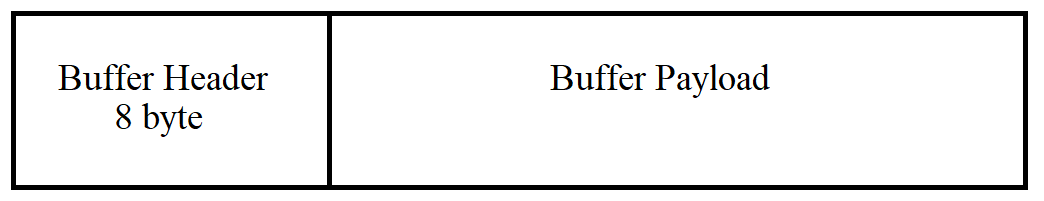
\includegraphics[width=\textwidth]{buffer}   
    Figure 1: Stuttura del buffer di invio di messaggi al server
\end{center}

Poichè il client ogni volta che invia un messaggio al server si mette in attesa di ricevere un messaggio di risposta da quest'ultimo (quindi i pacchetti da parte del 
client vengono inviati in maniera sequenziale), il server non ha bisogno di inviare al client l'id del pacchetto perché il client conosce già il tipo di pacchetto 
che sta per ricevere. Di conseguenza, il server invia prima la dimensione del pacchetto, poi il contenuto del buffer che vuole inviare. \\ In alcuni casi, se il server
non deve inviare nessun dato se non l'esito della richiesta che il client ha inviato, il server invia semplicemente un intero come messaggio di risposta:
nel caso di successo, il server invia 0, in caso di errore un numero negativo. 

\section{Server}

\subsection{Config}
Come richiesto dall'esame, il server all'avvio legge un file di configurazione con il seguente formato:

\begin{center}
    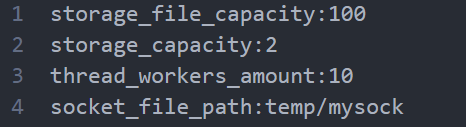
\includegraphics[width=80mm]{config} 
    \\Figure 2: Config.txt del server
\end{center}

Nel quale:
\begin{itemize}
    \itemsep 0em 
    \item \textbf{storage\_file\_capacity}: definisce il numero massimo di file che possono essere inseriti nello storage.
    \item \textbf{storage\_capacity}: definisce la dimensione massima in MB dello storage.
    \item \textbf{thread\_workers\_amount}: definisce il numero di thread workers.
    \item \textbf{socket\_file\_path}: definisce il percorso in cui creare il file socket.
\end{itemize}

\subsection{Struttura del Server}

Il server adotta come politica di rimpiazzamento dei file la politica \textbf{FIFO}, in cui il primo file ad entrare, è anche il primo file ad uscire dallo storage. All'avvio,
il server legge il file config sopra citato e successivamente avvia i seguenti thread:

\begin{itemize}
    \itemsep 0em 
    \item \textbf{Thread Signal Handler}: si occupa di gestire la ricezione dei segnali attraverso l'utilizzo del metodo \textbf{sigwait()}, in caso di ricezione di un segnale di 
    \textit{SIGINT}, \textit{SIGQUIT} o \textit{SIGHUP} il server termina correttamente l'esecuzione del programma come richiesto dall'esame.
    \item \textbf{Thread Dispatcher}: si occupa di accettare le nuove connessioni da parte dei client e delega le loro richieste ad una pool di \textit{Thread Worker}.
    \item \textbf{Thread Workers}: un insieme di thread che si occupano di eseguire le richieste dei client in maniera concorrente sullo storage del server.
\end{itemize}

Nel progetto sono state utilizzate due pipe:
\begin{itemize}
    \itemsep 0em 
    \item \textbf{pipeHandleClient}, utilizzata per inserire nuovamente il file descriptor all'interno del Thread Dispatcher dopo che il Thread Worker ha terminato l'esecuzione del task richiesto.
    \item \textbf{pipeHandleConnection}, è usata per terminare l'esecuzione del Thread Dispatcher quando viene inviato uno dei segnali di terminazione. Il Thread Signal Handler
    riceve il segnale, tramite la pipe comunica con il Thread Dispatcher (che è fermo in attesa di ricevere nuove richieste sul metodo \textbf{select()}) e notifica al Thread Dispatcher di
    terminare la propria esecuzione. Nel caso di un \textit{SIGINT} o \textit{SIGQUIT}, il Thread Dispatcher termina istantaneamente. Nel caso di un \textit{SIGHUP} il Thread Dispatcher tiene traccia di tutte
    le connessioni aperte tramite un contatore, quando il numero delle connessioni aperte diventa 0, termina l'esecuzione.
\end{itemize}

\subsection{Server Storage}

Lo Storage del server è stato implementato come una mappa attraverso l'utilizzo della libreria \textbf{icl\_hash.h}, ed ha:
\begin{itemize}
    \itemsep 0em 
    \item come chiave: il file, definito da una struct.
    \item come valore: la lista di tutti gli utenti che hanno richiesto l'operazione di open su quel file. 
\end{itemize}

La struct del file è formata da:
\begin{itemize}
    \itemsep 0em 
    \item \textbf{filePath}: il percoso assoluto del file.
    \item \textbf{fileContent}: il contenuto del file. 
    \item \textbf{fileSize}: la dimensione del file in byte.
    \item \textbf{fifo}: utilizzato dalla politica di rimpiazzamento FIFO. Ogni volta che un nuovo file viene creato, il server gli assegna un
    un valore univoco ed incrementale (per esempio il primo file avrà come valore 0, il secondo 1, etc.). Durante la politica di rimpiazzamento, il server sceglie
    come vittima il file che ha il valore fifo più basso e poi lo rimuove dallo storage.
    \item \textbf{fileLock}: lock utilizzata dai Thread Workers per eseguire le operazioni sul server in mutua esclusione. Ogni volta che un thread deve effettuare delle
    operazioni su un file già inserito nella mappa (per esempio aggiungere un nuovo utente alla lista o la modifica del contentuo del file), il Thread Worker deve prima acquisire
    la lock sul file, eseguire il task e poi rilasciarla a termine dell'operazione.
\end{itemize}

\begin{center}
    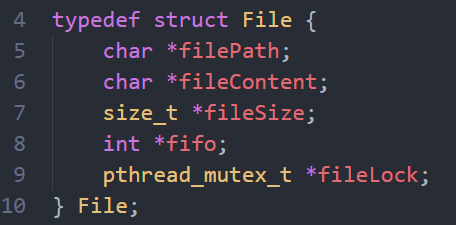
\includegraphics[width=80mm]{file}   
    \\Figure 3: Struct del file
\end{center}

\subsection{Lock}
Per rispettare la concorrenza e l'atomicità nel Server Storage, sono state utilizzate le seguenti lock:
\begin{itemize}
    \itemsep 0em 
    \item \textbf{StorageLock}: lock globale su tutta la mappa, viene utilizzata per inserire un nuovo file all'interno della struttura dati.
    \item \textbf{CapacityLock}: lock utilizzata per modificare in mutua esclusione il numero di file presenti nel server e la dimensione totale dello storage. 
    \item \textbf{ReplacementFrequencyLock}: lock utilizzata per contare in mutua esclusione quante volte è stata chiamata la politica di rimpiazzamento (per stampare il resoconto del server a fine esecuzione).
    \item \textbf{fileLock}: lock del file, utilizzata per modificare in mutua esclusione un file già presente all'interno della mappa.
\end{itemize}

\section{Client}

Come già spiegato, il client per comunicare con il server utilizza la libreria \textbf{client\_network.h} che si occupa di aprire la connessione sul server tramite socket e di
comunicare con il server utilizzando il protocollo spiegato precedentemente. \\ 
Il client per eseguire una qualsiasi operazione su un file del server deve prima eseguire la richiesta
di open su quel file, eccetto per la richiesta di \textbf{readN()} dato che non è possibile conoscere il numero preciso di file che l'utente andrà a leggere. Di conseguenza, 
un utente può eseguire la remove o la close di un file soltanto se prima ha richiesto la open su di esso. \\
Quando un utente si disconnette, il server rimuove in mutua esclusione (tramite \textbf{fileLock}) il file descriptor dell'utente disconnesso da ogni lista della mappa,
se presente. In questo modo, se un nuovo utente si connette al server e ottiene lo stesso file descriptor dell'utente disconnesso precedentemente, il nuovo utente non avrà
nessuna richiesta di open già eseguita.
\\[8pt]
Come richiesto dal testo dell'esame, il client può inviare differenti richieste al server passando i comandi per argomento. Per poter ricevere i comandi in qualsiasi ordine 
(quindi non è necessario che il primo comando da passare al client è \textit{-f}), quest'ultimi vengono inseriti all'interno di una lista monodirezionale. Successivamente, il client
prima controlla la presenza degli argomenti: \textit{-h}, \textit{-p}, \textit{-t}, \textit{-d} e \textit{-f}, se questi vengono trovati allora il client li esegue,
li rimuove dalla lista e poi esegue tutti i comandi rimasti nello stesso ordine di inserimento.

\end{document}